\documentclass{sig-alternate}
\usepackage{textcomp}
\usepackage{graphics}
\pagestyle{plain}
\usepackage{subfigure}
\usepackage[margin=10pt,font=small,labelfont=bf, labelsep=endash, skip=0pt]{caption}
\usepackage[latin1]{inputenc}
\usepackage{listings}

\begin{document}

\pagenumbering{arabic}

\title{Mahjong Solitaire}
\subtitle{Sistemas de Inteligencia Artifical - ITBA}

\numberofauthors{3}

\author{
	\alignauthor{Carlos Sessa}\\
	\alignauthor{Lucas Pizzagalli}\\
	\alignauthor{Nicol\'as Purita}\\
}

\date{09 de Mayo de 2011}

\maketitle

\section*{Introducci\'on}
	Se implementa un \textit{Sistema de Producci\'on} el cual es utilizado para resolver un juego denominado \textbf{Mahjong-Solitaire}, tambi\'en conocido como el \textit{Taipei}. Se utiliza un motor de inferencia en \textit{Java} para la resoluci\'on del problema designado, el cual fue entregado por la c\'atedra. \\
	Como punto de partida para crear el \textit{Sistema de Producci\'on} se dise\~{n}a un sistema de almacenamiento apropiado que represente el problema de la forma m\'as \'optima. Se utilizan 3 estrategias de b\'usqueda no informadas para comparar las distintas soluciones alcanzadas, las cuales se detallan en el transcurso del informe.

\section*{Reglas del Mahjong-Solitaire}
	El juego \textbf{Mahjong-Solitaire} consiste en eliminar todas las fichas de un tablero que posee 144 fichas. \\
	Las fichas deben ser removidas de a pares y solo si cumplen con las siguientes condiciones: No deben encontrarse bloqueadas y el par debe estar compuesto por fichas que sean del mismo tipo, y posean el mismo identificador. Las fichas existentes son:


\begin{table}[h]
\begin{center}
	\begin{tabular}{|c|c|c|}
	\hline
	 Tipo de Ficha & Identificador & Cantidad\\
	\hline \hline
	\textit{Character} & 9 & 4 de c$\setminus$u \\
	\textit{Bamboo} & 9 & 4 de  c$\setminus$u  \\
	\textit{Circles} & 9 & 4 de  c$\setminus$u  \\
	\textit{Dragons} & 3 & 4 de  c$\setminus$u  \\	
	\textit{Winds} & 4 & 4 de  c$\setminus$u  \\
	\textit{Season} & 4 & 1 de c$\setminus$u \\
	\textit{Flowers} & 4 & 1 de  c$\setminus$u  \\
	\hline
	\end{tabular}
\end{center}
\caption{Distribuci\'on de fichas}
\label{tab:tiles}
\end{table}

	Existe una excepci\'on en la remoci\'on de las fichas del tipo \textit{Season} o \textit{Flowers}. La excepci\'on esta basada en que cualquier ficha de \textit{Season} o \textit{Flowers} puede ser removida en conjunto con otra del mismo grupo por m\'as que no sea igual. Ejemplo: Summer con Winter. \\
	Una ficha bloqueada puede estar en forma \textit{Horizontal}, \textit{Vertical} o \textit{Ambos}. Estos bloqueos se definen del siguiente modo:
	\begin{itemize}
		\item \textbf{Horizontal}: La ficha elegida posee una ficha a su izquierda y derecha.
		\item \textbf{Vertical}: La ficha elegida posee una ficha encima de ella (tanto parcial como totalmente).		
	\end{itemize}
	En la Figura \ref{fig:blocking} se puede observar distintas posibilidades de bloqueos.\\
	Es muy importante destacar, que no todos los tableros tienen una soluci\'on, sino que la distribuci\'on de las fichas debe ser especialmente dise\~nada con tal objetivo. Por ejemplo, es posible crear tableros recorriendo el camino inverso que al resolver el mismo (ir colocando de a pares las fichas en lugares no bloqueados).
\section*{Desarrollo}

	Se representa un estado del juego como un vector de vectores en donde cada celda posee una \textit{Tile}. Este vector de vectores es del tipo:
	\begin{itemize}
		\item \textit{Tile}[a][b][c]
	\end{itemize}
	donde \textit{a} indica el nivel en el que se encuentra la ficha, \textit{b} es la fila y \textit{c} la columna. La clase \textit{Tile} est\'a definida como la composici\'on de un tipo de ficha y un n\'umero.
	
\section*{Funciones de costo}

	Dado que el objetivo del juego es simplemente retirar todas las fichas del tablero, y las mismas deben ser retiradas siempre de a pares, la funci\'on de costo propuesta es constante, haciendo referencia a la remoci\'on de un par del tablero. Dicha funci\'on se denomina \textit{$g_1$}. \\
	
	\section*{Heur\'isticas}

	Se considera \textit{Pair} a todo par de fichas con posibilidad de ser retiradas del tablero en un estado determinado y \textit{Payers} a la lista de dichos \textit{Pares}. \\
	Se proponen las siguientes heur\'isticas (para desarrollar en las estrategias de b\'usquedas no informadas):
	\begin{itemize}

		\item \textbf{M\'as Alta} \textit{(h1)}: Se libera el \textit{Pair} de m\'as alto nivel. En el mejor de los casos la remoci\'on de una ficha en una capa m\'as alta puede liberar cuatro fichas, lo cual aumenta la cantidad de \textbf{Payers} en la siguiente jugada.
		
		\item \textbf{Mayor cantidad de fichas horizontales} \textit{(h2)}: Esta heur\'istica busca reducir la posibilidad de eliminar una fila del tabler. La heur\'istica se basa en calcular la cantidad de fichas que posee cada fila en la que se encuentran cada ficha que compone el \textit{Pair} , esto se calcula como:
			\begin{eqnarray}
				X_{1}  & = & \# Fichas_{Fila de F_{1}} \\
				X_{2}  & = & \# Fichas_{Fila de F_{2}} \\
				\textbf{h2} & = & (\#FichasTot - ( X_{1} + X_{2} )) / 2
			\end{eqnarray}
		donde $F_{1}$ y $F_{2}$ son las fichas que componen el \textit{Pair}. Esta heur\'istica puede ser mejorada para priorizar le remoci\'on de las fichas de niveles superiores agregando un modificador seg\'un el nivel en que se encuentre, por ejemplo:
			\begin{eqnarray}
				\textbf{h2}  = (\#FichasTot. - ( X_{1} * N_{1} * C + X_{2} * N_{2} * C) )/ 2
			\end{eqnarray}
				donde $N_{1}$ y $N_{2}$ son los niveles de las fichas $F_{1}$ y $F_{2}$ respectivamente, y $C$ hace referencia a una constante la cual determina el grado de relevancia que se le quiera dar al nivel en que se encuentre la ficha (en nuestro caso 1) y es dividido por 2 para hacer referencia a pares en lugar de fichas. Es importante destacar, que se hacen todos los chequeos necesarios para que no sea negativa ni $0$ en caso erroneo.
		
		\item \textbf{Generador M\'aximo de \textit{Payers}} \textit{(h3)}: Esta heur\'isitca se basa en eliminar los \textit{Pairs} que generen mayor cantidad de \textit{Payers} en el pr\'oximo estado.
		
	\end{itemize}
	
\section*{Modificaciones en el motor de inferencia}
Con el objetivo de obtener amoldar el motor a los requerimientos de este problema en particular, y con el objetivo de aumentar su presici\'on, performance y flexibilidad se  le han introducido los siguientes modificaciones:
\begin{itemize}
	\item Se ha modificado de \emph{Integer} a \emph{float} el retorno de la funci\'on que devuelve la heur\'istica de un estado, con el objetivo de, por un lado evitar el boxing y unboxing de \emph{int} a \emph{Integer} y para lograr una mayor granularidad en las heur\'isticas.
	\item Se ha decidido modificar la funci\'on de costos tambi\'en para mantener correlaci\'on con la heur\'istica, aumentar la flexibilidad y hacer algunas pruebas con costos decimales.
	\item Se ha modificado la funci\'on encargada de retornar las reglas aplicables, al requerir un nuevo par\'ametro que representa el estado, para que la funci\'on solo devuelva las reglas aplicables en dicho estado. De esta forma se reduce mucho el set de reglas a aplicar, reduciendo la memoria y procesamiento requerido.
	\end{itemize}

\section*{Resultados y Conclusiones}
\subsection*{Algoritmos no informados}	
En la tabla \ref{tab:cost} se ven los distintos resultados para distintas estrategias de b\'usqueda	 en algoritmos no informados. \\
Debido, a que cualquier soluci\'on es \'optima y para llegar a la misma se debe alcanzar los nodos hojas, que se encuentran a una profundidad constante, la estrategia  \emph{DFS} es la m\'as \'optima, al expandirse primero hacia las hojas y luego a lo ancho. Por lo contrario, tanto \emph{BFS} y \emph{Profundizaci\'on iterativa} tienden a encontrar soluciones muy lentamente y en varios casos sin encontrar resultados debido a falta de memoria o time out. \\

\subsection*{Algoritmos informados}
Si bien el resultado general es m\'as alentador que con los no informados, siguen teniendo una similitud, al obtener mejores resultados los que se caracterizan por recorrer en profundidad tales como \emph{Greedy}, en contraposici\'on con los que tienden a expandir por nivel tales como \emph{$A^*$} como se puede observar en la tabla \ref{tab:costHeuristic}. A su vez, se puede observar que depende mucho de la heur\'istica utilizada. Por ejemplo, hay heur\'isticas que tienden a no ser muy buenas cuando se tiene un tablero grandes, pero que son superadas por otras cuando la cantidad de fichas se disminuye. Un claro ejemplo es como la \emph{h2} es muy buena en tableros grandes, pero que a medida que el tablero disminuye la cantidad de fichas presentes pierde terreno frente a las otras heur\'isticas hasta ser superada.\\
Otra dato a tener en cuenta, es el beneficio que se logra utilizando un algoritmo informado frente a los no informados. Otra vez, debido a la naturaleza del problema, es buena idea separar entre algoritmos que tienden a explorar por nivel (\emph{$A^*$}, \emph{BFS}, \emph{Profundizaci\'on Iterativa}) y los que tienden a ir  hacia las hojas (\emph{Greedy} y \emph{DFS}).\\
En el primer grupo, se puede observar como, si bien los algoritmos no informados se equiparan en performance a \emph{$A^*$} en tableros con pocas fichas, este \'ultimo los supera ampliamente en tableros m\'as complejos consiguiendo terminar para varias heur\'isticas en tiempos aceptables.\\
Para el segundo grupo de algoritmos, \emph{DFS} se comporta excelentemente debido a lo ya explicado anteriormente referido a su velocidad en alcanzar las hojas. Es por eso que no se ven mejoras tan marcadas como en el caso anterior. Sin embargo, se puede observar que \emph{Greedy} logra superarlo si se utilizan buenas heur\'isticas en tableros m\'as grandes (\emph{Greedy} utilizando la heur\'istica \emph{h2} tarda $30\%$ menos de tiempo y expande casi la mitad de nodos que \emph{DFS} en el tablero con 144 fichas) .\\
En resumen, para este problema, los algoritmos que mejor se desepe\~nan son aquellos que llegan r\'apidamente a las hojas, aumentando la eficiencia si se utilizan algoritmos de este tipo informados. Por otro lado, los algoritmos que se expanden por nivel tienden a tener una performance muy baja, especialmente con tableros con muchas fichas. Este problema puede ser mejorado parcialmente al aplicar algoritmos informados de este tipo con las heur\'isticas correctas.\\



\onecolumn

\begin{figure}[h!]
  \begin{center}
  	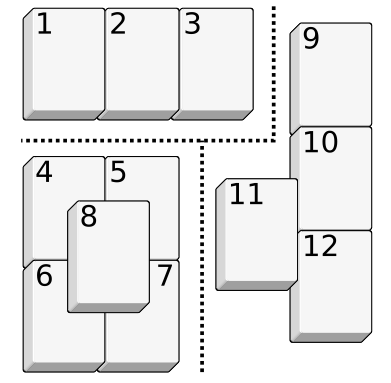
\includegraphics[scale=0.3]{images/blocking.png}
  \end{center}
  \caption{Ficha 2 es bloqueada por la 1 y 3. La ficha 4-7 est\'an bloqueadas por la 8. El resto de las fichas son movibles.}
  \label{fig:blocking}
\end{figure}

\begin{figure}[h!]
  \begin{center}
      \subfigure[Tablero 1]{\label{fig:layout1}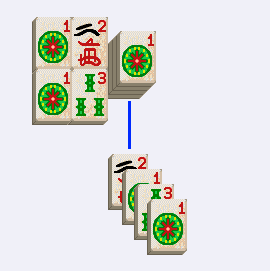
\includegraphics[scale=0.3]{Boards/Layout1.png}}
    \hspace{20pt}
    \subfigure[Tablero 2]{\label{fig:layout3}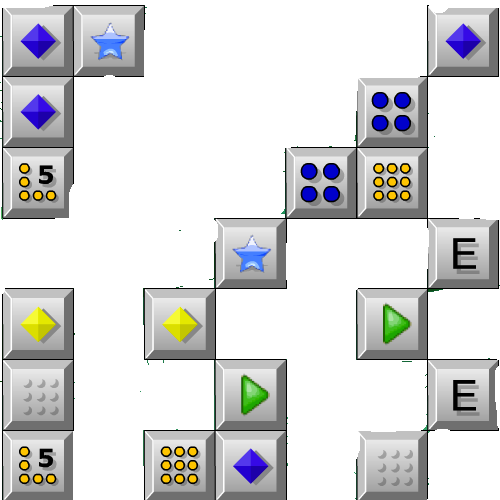
\includegraphics[scale=0.2]{Boards/Layout3.png}}
    \hspace{20pt}
    \subfigure[Tablero 3]{\label{fig:layout4}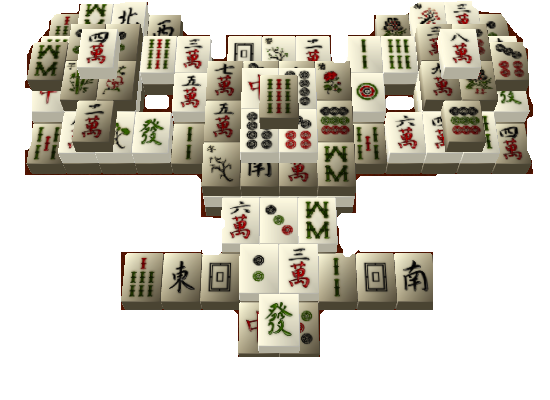
\includegraphics[scale=0.2]{Boards/Layout4White.png}}
  \end{center}
  \caption{Distintos tableros}
  \label{fig:layouts}
\end{figure}
	
	
\begin{table}[h]
\begin{center}
	\begin{tabular}{|p{2.3cm}|p{2cm}|p{2cm}|p{2cm}|p{2cm}|p{4cm}|}
	\hline
	 Algoritmo & Nodos expandidos & Nodos en la frontera & Nodos generados & Profundidad de la Soluci\'on & Tiempo de Procesamiento\\
	\hline \hline
		 \multicolumn{6}{|c|}{Layout 1} \\
	\hline
	\textit{DFS} & 6 & 0 & 6 & 4 & 32ms \\
	\textit{BFS} & 7 & 0 & 6 & 4 & 10ms \\
	\textit{Produndizaci\'on Iterativa} & 7 & 7 & 19 & 4 & 12ms \\
	\hline
		 \multicolumn{6}{|c|}{Layout 2} \\
	\hline
	\textit{DFS} & 11 & 57 & 10 & 10 & 74ms \\
	\textit{BFS} &5944 & 34491 & 5944 & ? & 5' \\
	\textit{Produndizaci\'on Iterativa} & 7550 & 33571 & 5696 & ? & 5' \\
	\hline
		 \multicolumn{6}{|c|}{Layout 3} \\
	\hline
	\textit{DFS} & 73 & 1438 & 72 & 72 & 2'' 708ms \\
	\textit{BFS} & 641 & 15705 & 641 & ? & 5' \\
	\textit{Produndizaci\'on Iterativa} & 620 & 14964 & 587 & ? & 5' \\
	\hline
	\end{tabular}
\end{center}
\caption{Resultados de resolver el problema de los tableros \ref{fig:layout1}, \ref{fig:layout3} y \ref{fig:layout4} con distintos algoritmos no informados}
\label{tab:cost}
\end{table}

\begin{table}[h]
\begin{center}
	\begin{tabular}{|p{2cm}|p{2.0cm}|p{2cm}|p{2cm}|p{2cm}|p{2cm}|p{4cm}|}
	\hline
	 Algoritmo & Heur\'istica & Nodos expandidos & Nodos en la frontera & Nodos generados & Profundidad de la Soluci\'on & Tiempo de Procesamiento\\
	\hline \hline
		 \multicolumn{7}{|c|}{Layout 1} \\
	\hline
	\textit{$A^*$} & h1 & 4 & 2 & 5 & 4 & 20ms \\
	\textit{$A^*$} & h2 & 4 & 2 & 5 & 4 & 14ms \\
	\textit{$A^*$} & h3 & 4 & 2 & 5 & 4 & 14ms \\
	\textit{Greedy} & h1 & 4 & 2 & 5 & 4 & 35ms\\
	\textit{Greedy} & h2 & 4 & 2 & 5 & 4 & 227ms\\
	\textit{Greedy} & h3 & 4 & 2 & 5 & 4 & 49ms\\
	 \hline \hline
		 \multicolumn{7}{|c|}{Layout 2} \\
	\hline
	\textit{$A^*$} & h1 & 10 & 57 & 11 & 10 & 130ms \\
	\textit{$A^*$} & h2 & 10 & 57 & 11 & 10 & 97ms \\
	\textit{$A^*$} & h3 & 5983 & 34934 & 5983 & ? & 5'\\
	\textit{Greedy} & h1 & 10 & 49 & 10 & 11 & 126ms\\
	\textit{Greedy} & h2 & 10 & 49 & 10 & 11 & 110ms\\
	\textit{Greedy} & h3 & 10 & 49 & 10 & 11 & 133ms\\
	\hline \hline
		 \multicolumn{7}{|c|}{Layout 3} \\
	\hline
	\textit{$A^*$} & h1 & 525 &  10660 & 525 & ? & 5' \\
	\textit{$A^*$} & h2 & 72 & 1438 & 73 & 72 & 2'' 864ms\\
	\textit{$A^*$} & h3 & 349 & 17903 & 349 & ? & 5' \\	
	\textit{Greedy} & h1 & 72 & 1121 & 73 & 72 & 2'' 502ms\\
	\textit{Greedy} & h2 & 72 & 857 & 73 & 72 & 1'' 812ms\\
	\textit{Greedy} & h3 & 72 & 2096 & 73 & 72 & 4'' 502ms\\
	\hline
	\end{tabular}
\end{center}
\caption{Resultados de resolver el problema de los tableros \ref{fig:layout1}, \ref{fig:layout3} y \ref{fig:layout4} con distintos algoritmos informados}

\label{tab:costHeuristic}
\end{table}

\end{document}